% This is part of Un soupçon de mathématique sans être agressif pour autant
% Copyright (c) 2014
%   Laurent Claessens
% See the file fdl-1.3.txt for copying conditions.

\begin{exercice}\label{exosmath-0836}

    Voici \wikipedia{fr}{Pente_(topographie)}{un extrait de Wikipédia} :\\
    \boxed{
    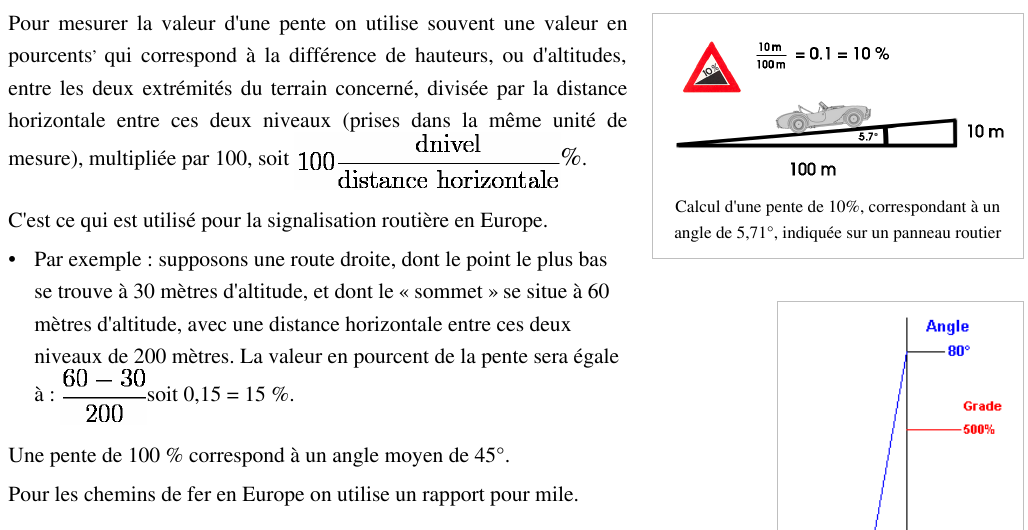
\includegraphics[width=\linewidth]{pente_pourcent.png}
}
Pour votre culture générale, remarquez que les accents dans la formule \( 100\dfrac{ \text{dénivelé} }{ \text{distance horizontale} }\%\) ne sont pas passés.

\begin{enumerate}
    \item
        Expliquer pourquoi une pente à \SI{45}{\degree} correspond à une pente de \( 100\%\).
    \item
        Une route de \SI{5}{\kilo\meter} monte un dénivelé de \SI{1}{\kilo\meter}. Quel est le pourcentage de la pente ?
\end{enumerate}

\corrref{smath-0836}
\end{exercice}
